\chapter{Force Estimation}
In order to have a representation of the reaction force on the EndoWrist, estimation is needed.
Because of the reasons mentioned in chapter \ref{introduction}, the force cannot be measured real-time using sensors and thus we have to rely on mathematical models as functions of actuator measurements.

The main challenge faced in making a model lies in the fact that the pulley system on the EndoWrist is nonlinear, and thus its full dynamics cannot be modeled in a straightforward manner. 
In other words, to have an accurate representation of Cartesian force a higher order model is required.

Another method of tackling this problem is to create multiple mathematical models pertaining to forces output by actions performed with the EndoWrist.
In this manner, the feedback vector is transformed from Cartesian space to a task space in which the chosen actions form a basis.
Each element of the new feedback vector corresponds to an actuated axis of the Geomagic Touch.
For the purpose of this system, we choose to feedback the yaw force generated by the grip action of the clamp, the torque generated by the roll actuator and force exerted by the clamps pitch movement.

\section{System Identification}
System identification is performed by fitting input and output data of the system to a known (grey-box) or unknown (black-box) mathematical model, generated either using theoretcal knowledge or data-fitting algorithms. 
This is done by changing the parameters of the model in a way that increases some measure of the quality of the model.

For our project, we require our model to output a measure of the force exerted by the EndoWrist.
Ideally a mathematical model derived from classical mechanics would be used to describe the dynamics involved in EndoWrist movement.
However, deriving this model precisely enough for grey-box identification has been proven difficult and time consuming due to the nonlinear nature of the dynamics \cite{kim2014dynamic}.

The nonlinearity of EndoWrist dynamics emerges from friction forces between the pulley strings controlling the end-effector, which causes multiple pulleys to move in cases where we only want to move one. 
Also, the strings themselves are elastic, which adds another dimension of nonlinearity.

For these reasons it was decided to test out different black box identification algorithms which only provide a general model structure where parameters don't have any physical meaning. Parameters are then identified using different variations of these algorithms and checked for accuraccy.

The system identification proces used in this project can be described in three steps:
\begin{enumerate}
\item Picking a model structure
\item Identifying parameters
\item Model validation
\end{enumerate}

\subsection{Model structure}
The first choice regarding model structure pertains to linearity.
Since our system is nonlinear , a straightforward approach would involve choosing a nonlinear model structure for identification.
On the other hand, stability analysis of nonlinear models is difficult and due to the nature of the system only general trends in force need to be represented.
For this reason it was decided to identify a linear state-space model which is then used as a part of Hammerstein-Weiner nonlinear model \cite{zhu2002estimation}.

A state-space model separates the dynamics of a system into a set of first-order differential equations.
Additionally, if the dynamical system is linear, time-invariant, and finite-dimensional, then the differential and algebraic equations may be written in matrix form. The general structure of such models is presented in equations \ref{eq:ssc}and \ref{eq:ssd} for the continous and discrete variants, respectively.

\begin{align}\label{eq:ssc}
\dot{\mathbf{x}} &= \mathbf{A}\mathbf{x} + \mathbf{B}\mathbf{u} \\
\mathbf{y} &= \mathbf{C}\mathbf{x} + \mathbf{D}\mathbf{u}
\end{align}
\vspace{-0.5cm}
\begin{align}\label{eq:ssd}
\mathbf{x}(k+1) &= \mathbf{A}\mathbf{x}(k) + \mathbf{B}\mathbf{u}(k)\\
\mathbf{y}(k+1) &= \mathbf{C}\mathbf{x}(k) + \mathbf{D}\mathbf{u}(k)
\end{align}

This representation of a system is especially useful in MIMO systems as it maintains the same form for any number of inputs and outputs, as opposed to transfer functions.

An identified state-space model can then be used as the linear part of an Hammerstein-Weiner model.
Hammerstein-Wiener models are useful when the output of the system depends nonlinearly on it's inputs, in this case it is possible to decompose the system into linear and nonlinear parts, as seen in \figref{weiner}. 
The nonlinearity estimators at the inputs and outputs of the system can be modeled by a variety of nonlinear systems, such as deadzones, saturations or even neural networks.

\begin{figure} 
\resizebox{\textwidth}{!}{
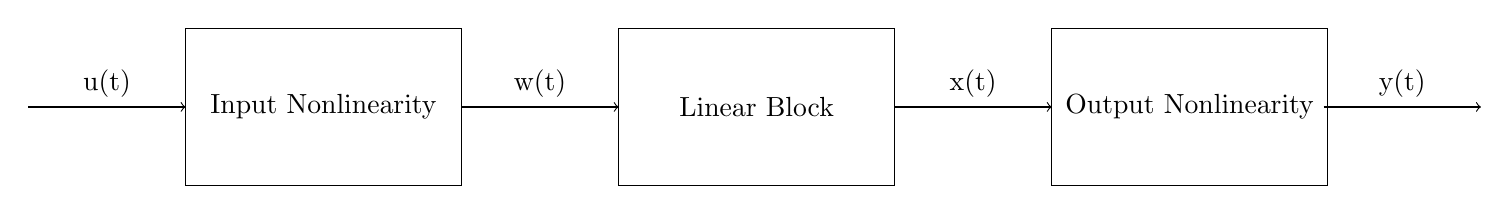
\begin{tikzpicture}
\draw  (-3.5,3) rectangle (0,1) node[pos=.5] {Linear Block};
\draw  (-9,3) rectangle (-5.5,1) node[pos=.5] {Input Nonlinearity};
\draw  (2,3) rectangle (5.5,1) node[pos=.5] {Output Nonlinearity};
\draw [->] (-5.5,2) -- (-3.5,2) node [pos=0.5,above] {w(t)};
\draw [->] (-11,2) -- (-9,2) node [pos=0.5,above] {u(t)};
\draw [->] (0,2) -- (2,2) node [pos=0.5,above] {x(t)};
\draw [->] (5.45,2) -- (7.45,2) node [pos=0.5,above] {y(t)};
\end{tikzpicture}
}
\caption{Block diagram of a Hammerstein-Wiener model\ref{fig:weiner}}
\label{weiner}
\end{figure}

A deadzone nonlinearity on the input allows us to represent the effects of friction on the force, and is used in this model.
Different output nonlinearities are also utilized and compared.

Two approaches were chosen in the matter of inputs and outputs of the model.
The first approach considered the possible correlation between the motor velocity and end-effector force during impact, so a model that outputs both force and velocity as a function of current could be corrected (as an observer) with actual velocity measurements and provide correction of the force model.
The second approach has the models output force as a function of current and velocity and thus cant be corrected.

The same modeling process was used for both the yaw and pitch models, while the roll model is explained in section \ref{se:mdval}.
For clarity, the results of each step in the process will only be presented for the yaw model, while the final results will be presented for both the yaw and pitch models.

\section{Parameter identification}
Once a general model structure has been chosen, parameter identification algorithms can be utilized.

For parameter identification to be performed on the Hammerstein-Weiner model, a linear model needs to be defined.
This means that it is first neccessary to identify the linear state-space model of the system.
Linear state space model fitting can be done using various methods , but for this purpose we have chosen the subspace identification algorithm.

Subspace identification is an algorithm that combines concepts from system theory, linear algebra and statistics in order to provide a state-space model of the system, which makes it useful for MIMO system identification \cite{van2012subspace}. 
The most important achievement subspace identification is based on is that Kalman filter states can be obtained from input-output data using linear algebra.
Although the algorithm itself is complex, it is implemented in the System Identification Toolbox as a part of MATLAB.

One advantage of subspace identification algorithms is the ability to estimate how much of the data dynamics a state-space model of a certain order can represent. 
As seen on figure (), the diminishing returns of increasing the state-space order are visible for different subspace identification algorithms.

%figure of subspace singular value analysis

\subsection{Identification data}
Both of these approaches are possible to realize on the data sets acquired in the manner described in chapter (measurement).
However, the data contains various irregularities caused by the imperfect measuring process as well as the hardware.
For this reason parts of the data needed to be removed before identification, which required interpretation of restults.
Also, linear model identification showed the best results when done on data in which the strongly nonlinear effects of friction were "cropped".

%figure showing shitty data

Noise is also present and can be removed from the identification data using a low pass filter.
Since most of the dynamics are captured in the frequency band of 0 to 20 rad-1 , this frequency range was chosen for identification.
Also, it is useful to remove the offsets (means) on output data.
A sample of original and modified data can be seen on \figref{figlowpass}.
%example of data
%\input{rapport/pictures/lowpass}
\begin{figure}[H]
\centering
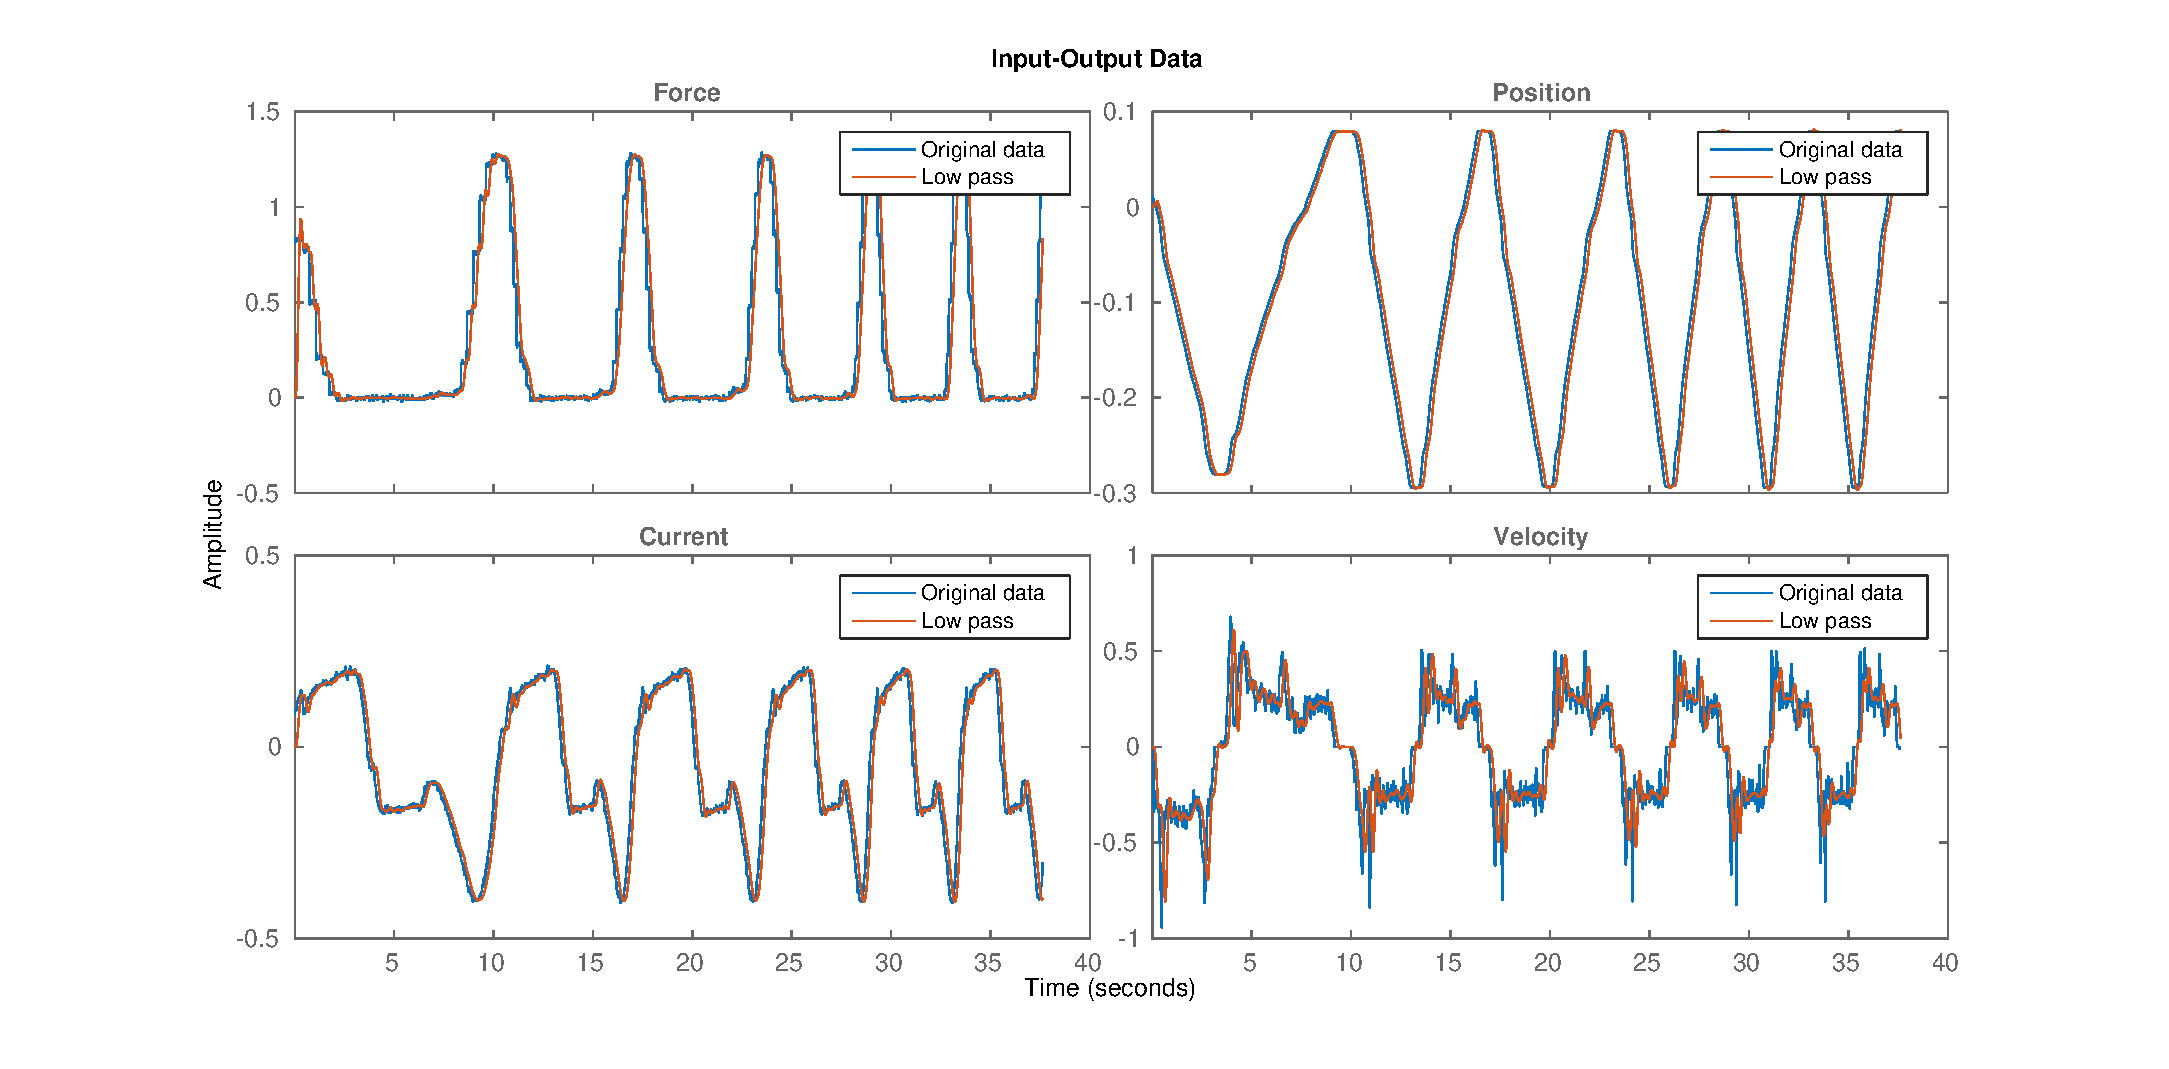
\includegraphics[width=1\linewidth]{lowpass.eps}
\caption{Comparison of original and low-pass filtered data.}
\label{figlowpass}
\end{figure}

\subsection{Linear model identification}

The System Identification Toolbox provides 3 different subspace identification algorithms which often provide different results depending on the chosen system order \cite{van1994n4sid}. 
For this reason all 3 algorithms are attempted in the identification process, and the best one is chosen depending on the average fit.
The algorithm which provides the best result varies heavily on the data set and the chosen order of the model.

%example of model fits to data
\begin{figure}[H]
\centering
\hspace{-2em}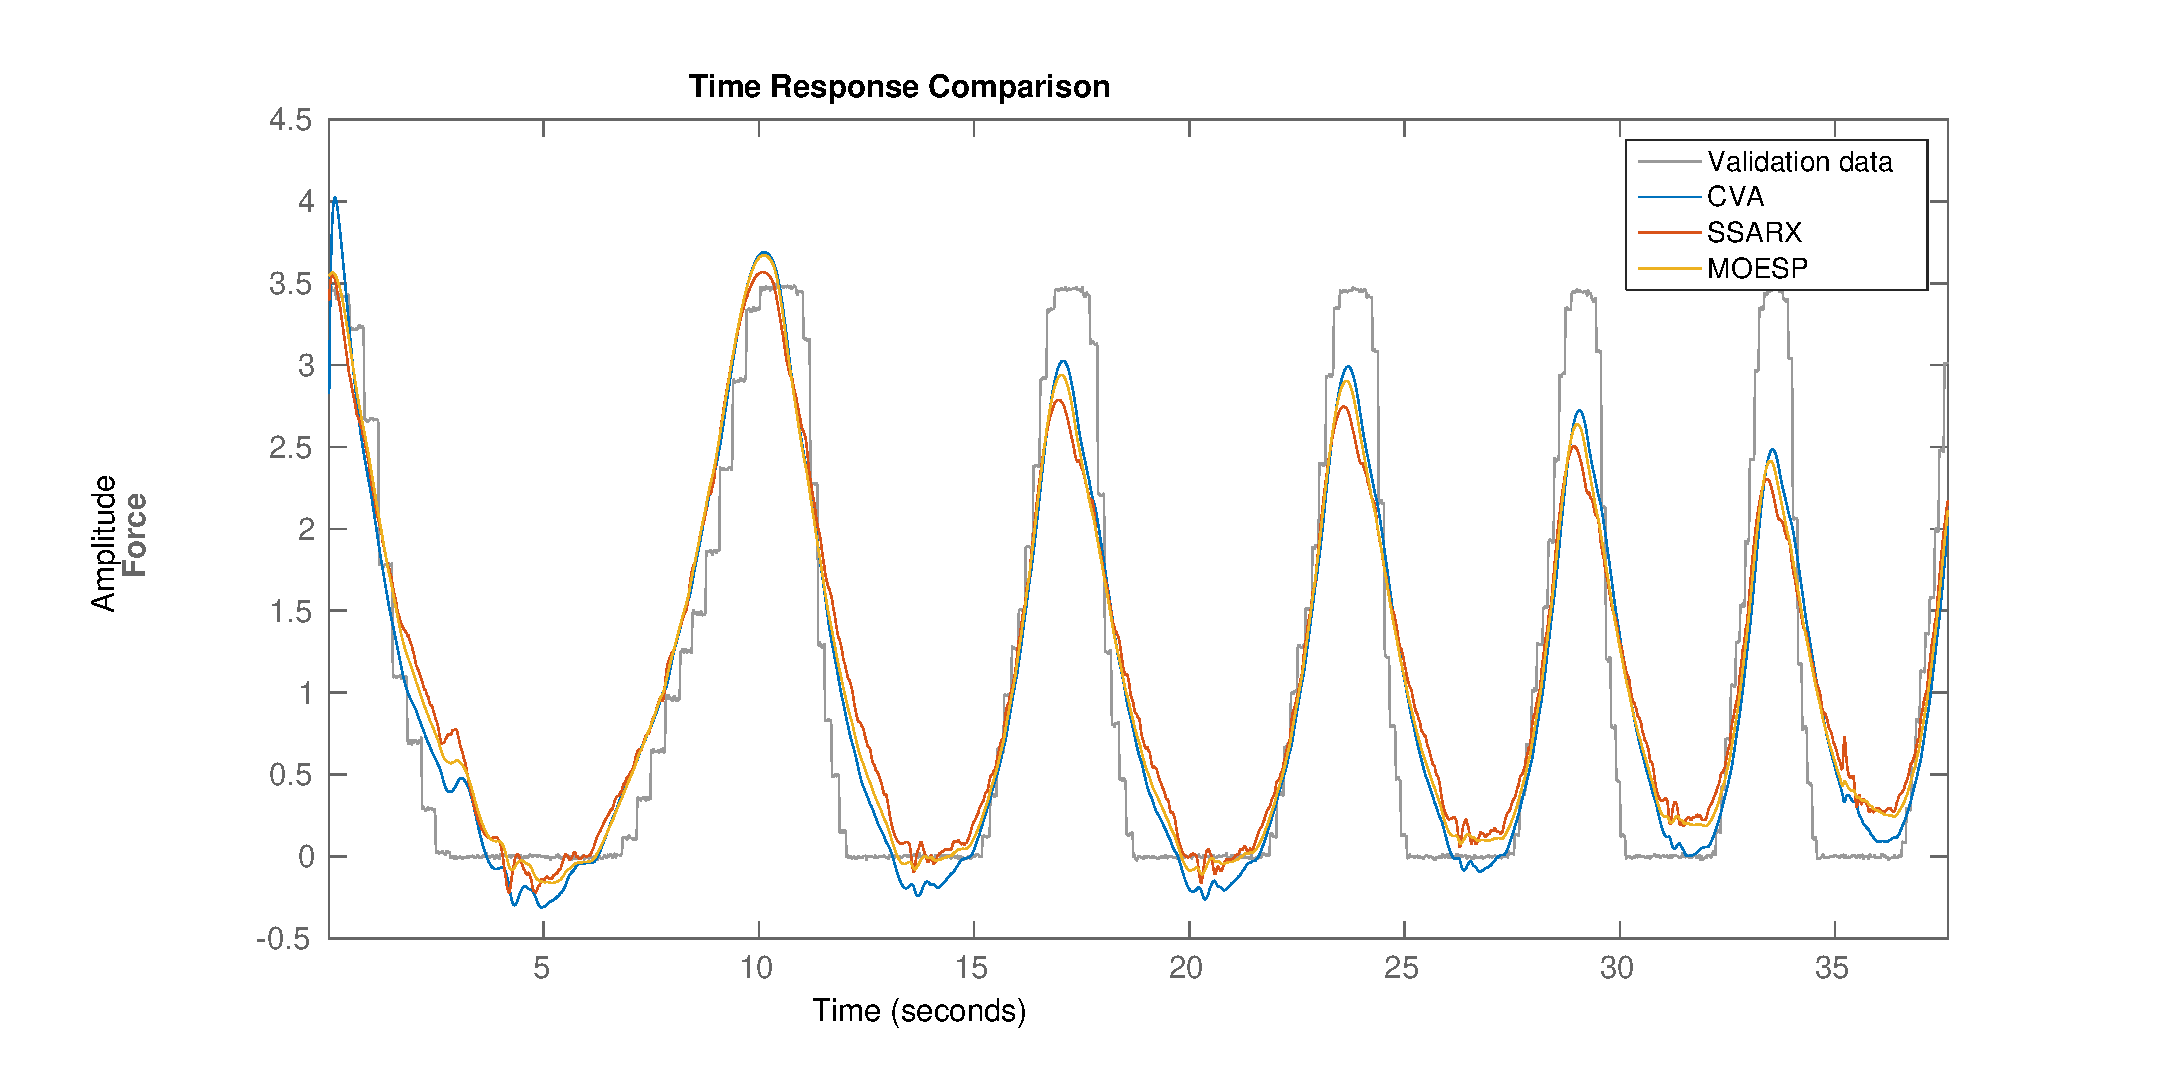
\includegraphics[width=0.7\linewidth]{sscomparison1}
\caption{Second order yaw force models identified by different subspace identification algorithms.}
\label{fig:1LMI}
\end{figure}



Comparing the responses of these models it is clear that having current and velocity as inputs provides a much better estimate than when the only input is effort.

\begin{figure}[H]
\centering
\hspace{-2em}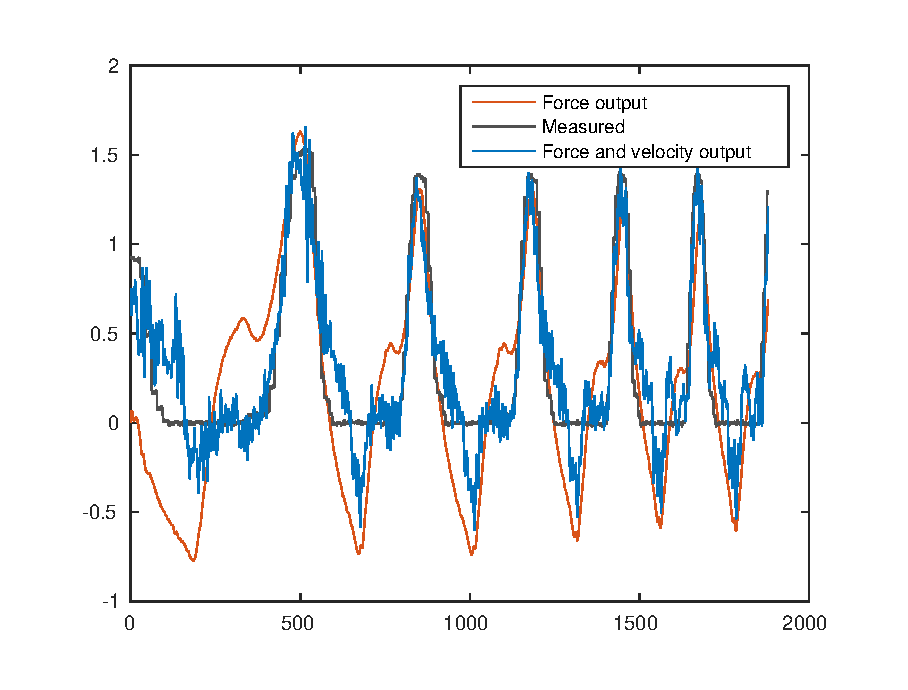
\includegraphics[width=0.7\linewidth]{comparisonp1p2}
\caption{Second order yaw force models identified by different subspace identification algorithms.}
\label{fig:1LMI2}
\end{figure}
\subsection{Hammerstein-Weiner model identification}

Once the linear model is identified we can estimate the nonlinearities with the Hammerstein-Wiener model.

\begin{figure}[H]
\centering
\hspace{-2.5em}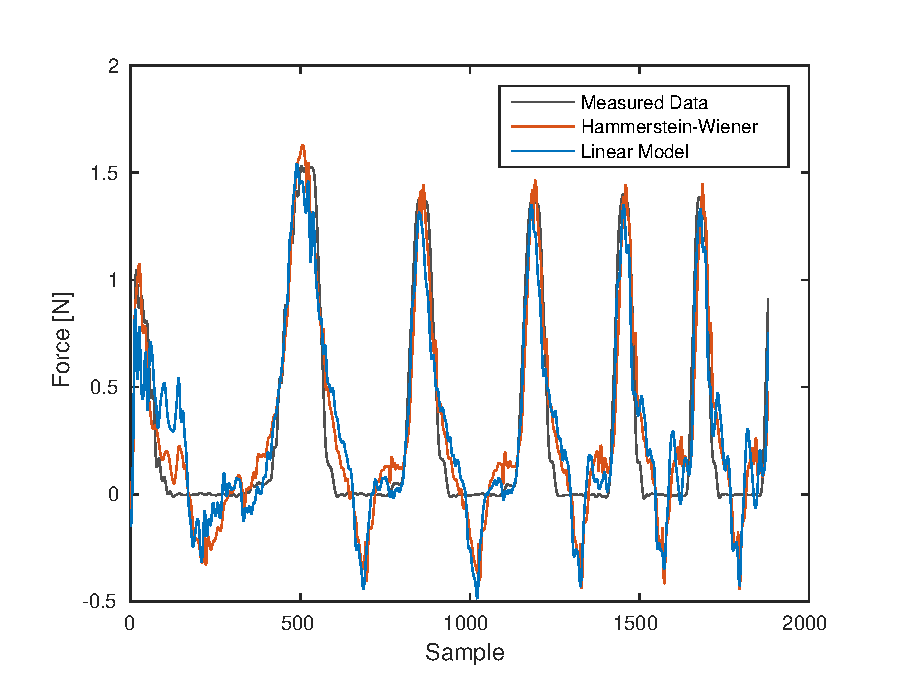
\includegraphics[width=0.7\linewidth]{sshwcomp1}
\caption{Hammerstein-Wiener model with deadzone nonlinearity responses compared to measured data for yaw force.}
\label{fig:2LMI}
\end{figure}

\begin{figure}[H]
\centering
\hspace{-2.5em}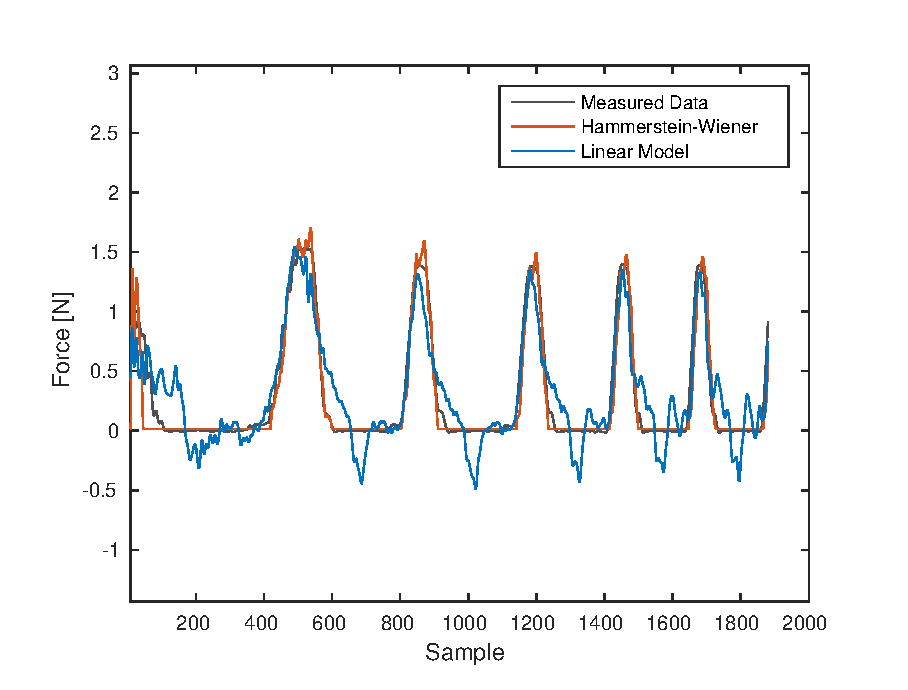
\includegraphics[width=0.7\linewidth]{sshwcomp2}
\caption{Hammerstein-Wiener model with deadzone input nonlinearity and saturation output nonlinearity responses compared to measured data for yaw force.}
\label{fig:2LMI1}
\end{figure}

\begin{figure}[H]
\centering
\hspace{-2.5em}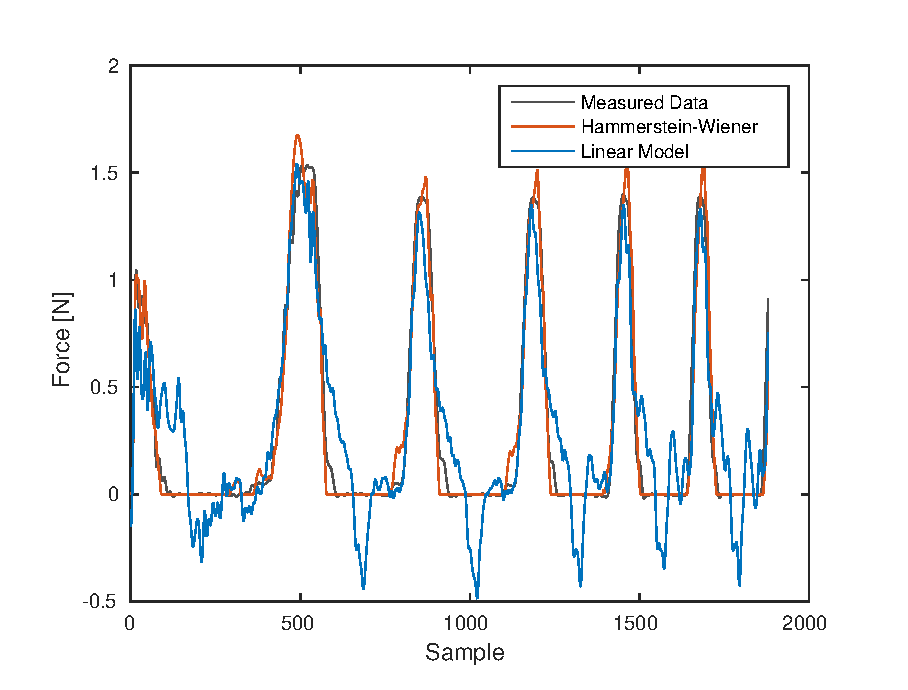
\includegraphics[width=0.7\linewidth]{sshwcomp3}
\caption{Hammerstein-Wiener model with deadzone nonlinearities on the output.}
\label{fig:2LMI2}
\end{figure}

It is noticable that the deadzone nonlinearity on the output significantly improves the linear model and as such makes for a good yaw force model.
This serves as a proof of concept for our own friction estimating nonlinearity based on measured data described in the control chapter.

\section{Model validation} \label{se:mdval}
Once a model has been created, it needs to be tested on data it wasn't originally fitted to for accuracy.
We expect our model to capture the general force dynamics in a way that is proportional to the actual force.
In that way we are able to represent the resulting force estimate as force feedback on the Geomagic Touch.

An important observation is that this model is fitted to dynamics of the clamp gripping the load cell, which has a hard surface.
It is expected that soft tissue would have a much smaller force gradient and thus it is expected that the model response overestimates the force slightly.
Nontheless, through the use of the system we came to a conclusion that the response is satisfactory for the degree of accuracy provided by the Geomagic Touch force feedback.

In figures \ref{fig:final_res_yaw} and \ref{fig:final_res_pitch} the response to different types of input data is examined.
The data was gathered in measurments described in CHAPTER, but wasn't used in the fitting process.


\begin{figure}[H]
\hspace{-2.5em}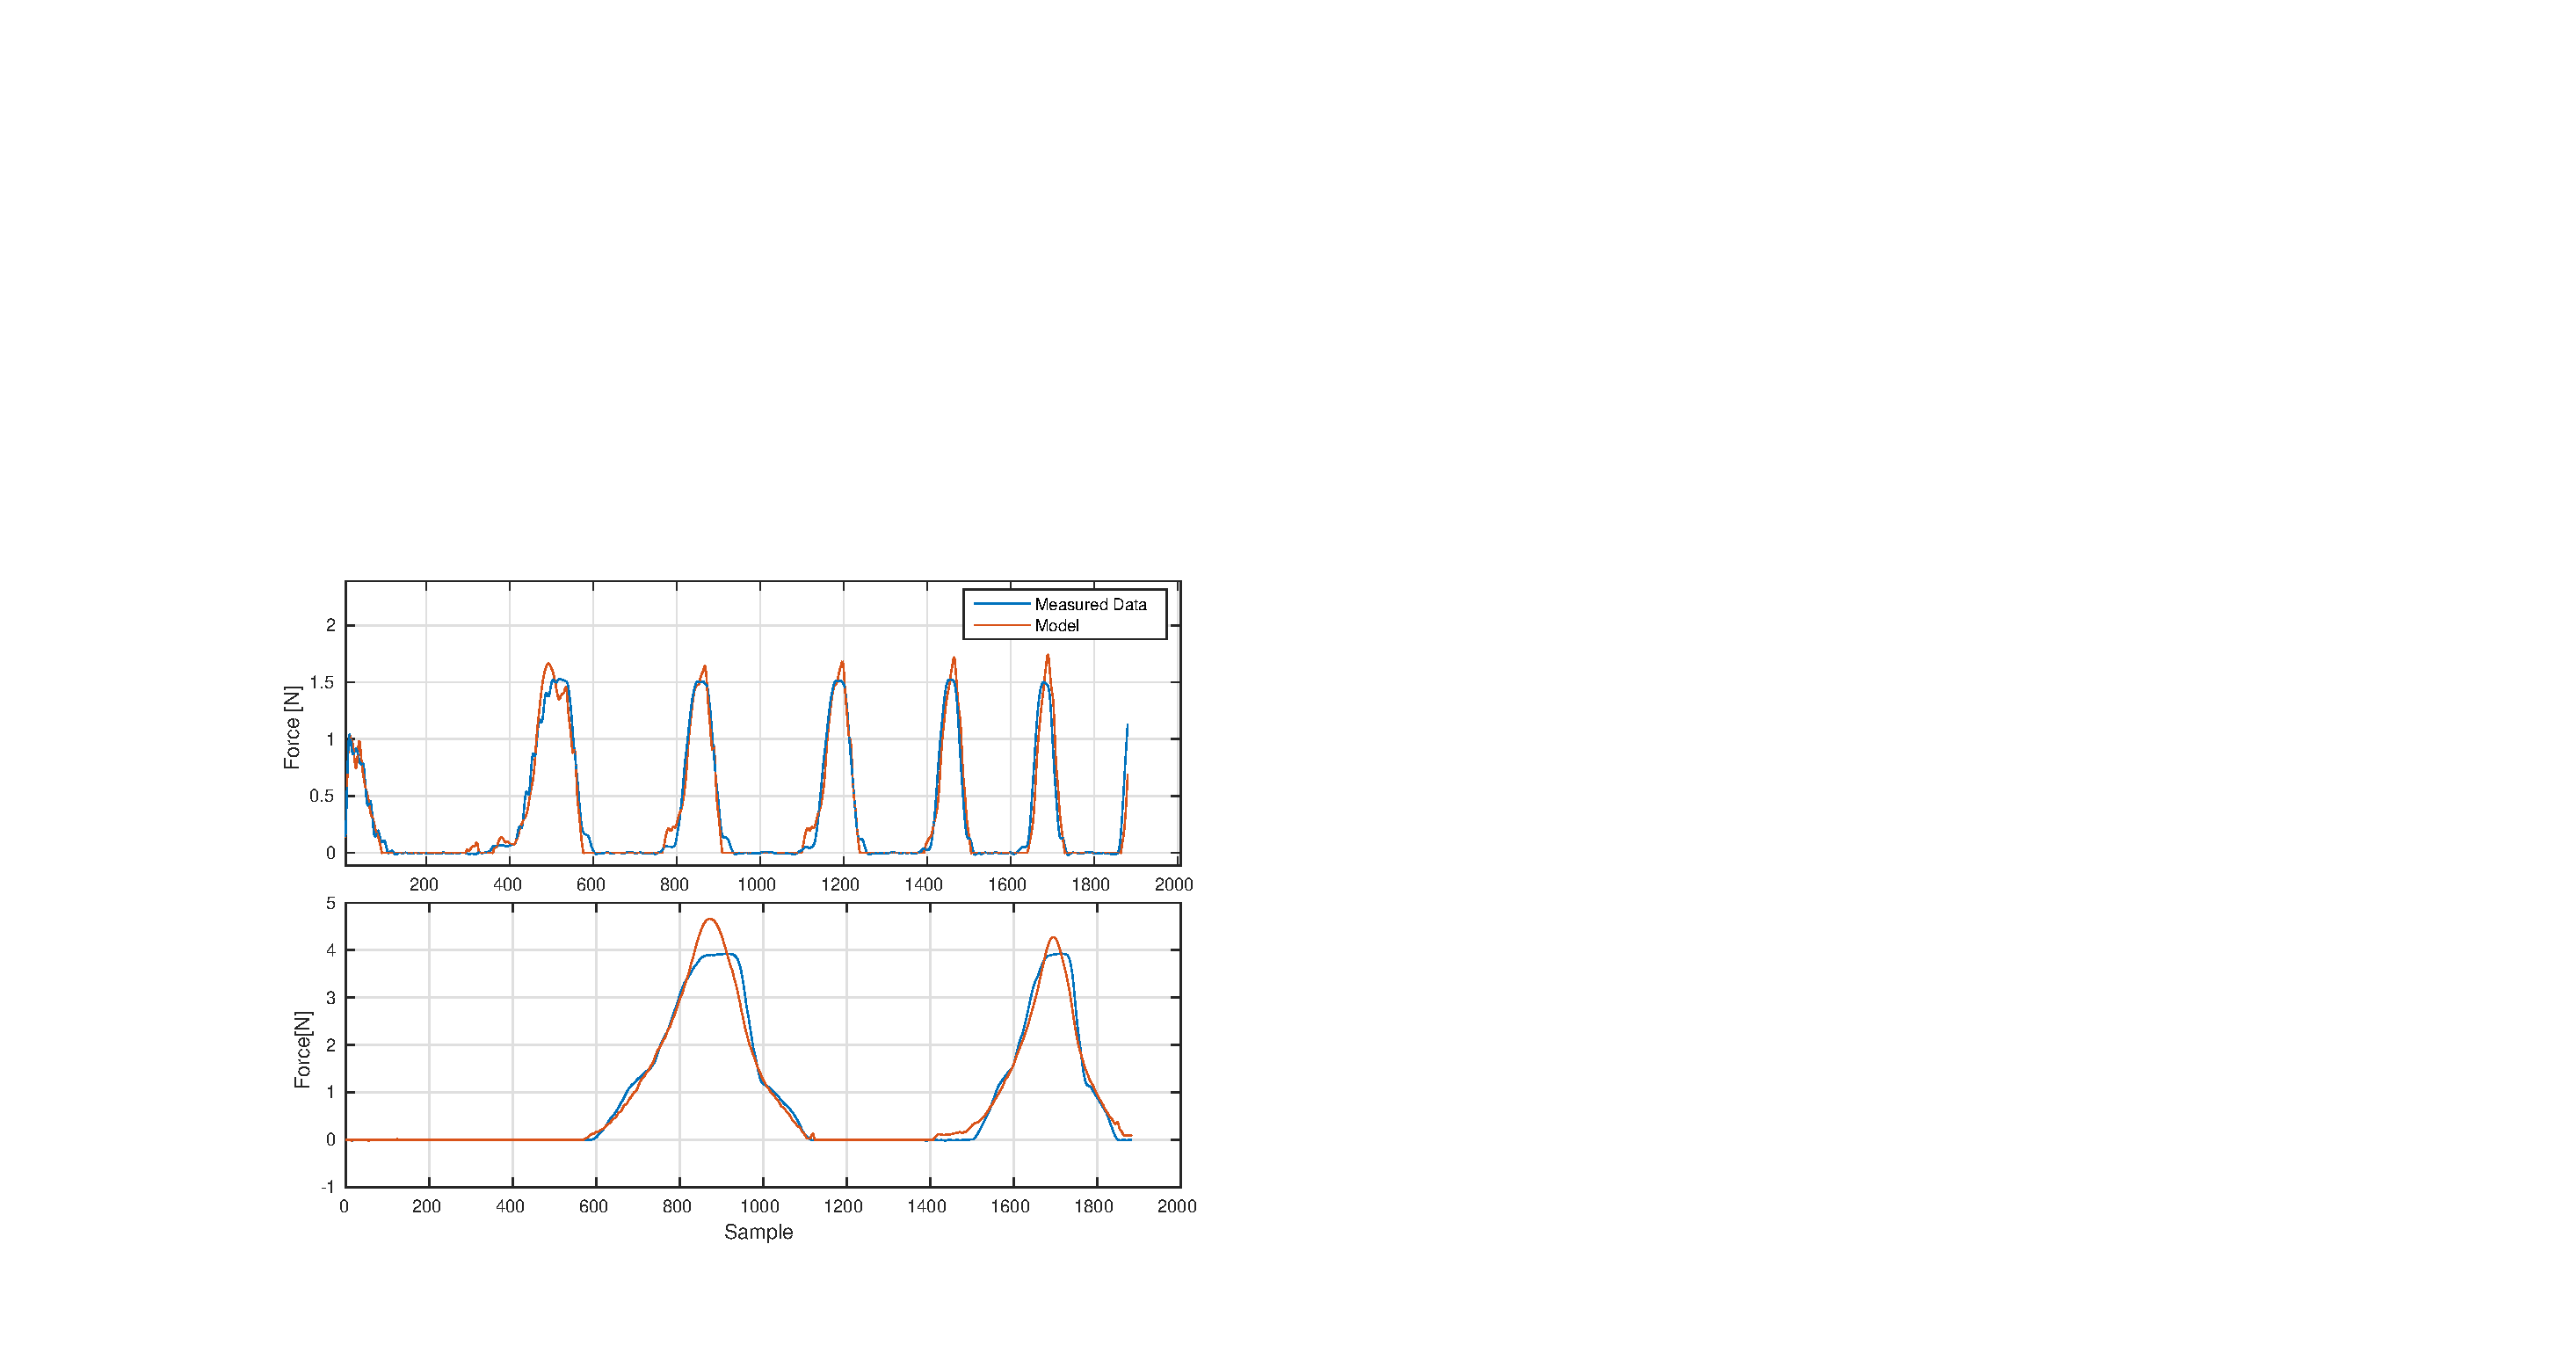
\includegraphics[width=1.2\linewidth]{modelyaw}
\caption{Yaw model excited with different types of inputs.}
\label{fig:final_res_yaw}
\end{figure}

Unlike the yaw model, the nonlinear pitch model had large jumps in value and was not useful for feedback.
Thus, the linear model is used.

\begin{figure}[H]
{-2.5em}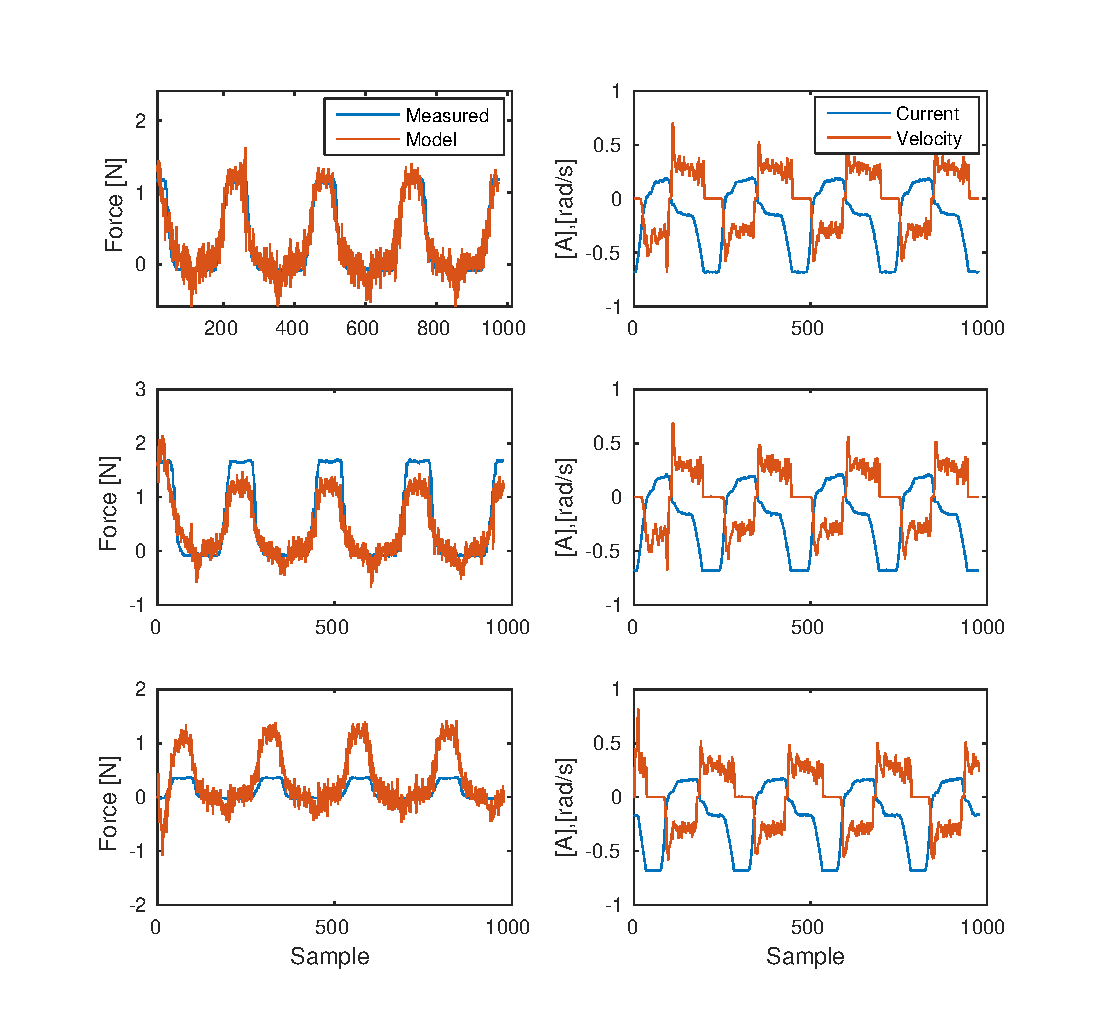
\includegraphics[width=1.2\linewidth]{modelpitch}
\caption{Pitch model excited with different types of inputs.}
\label{fig:final_res_pitch}
\end{figure}

The roll torque is an exception as it can be represented by a first level polynomial.
It is determined by the roll actuator and directly rotates the entire tool,.
This means we can make the assumption of linearity for the relation between the roll actuator effort and torque.  
By simple measurement with the setup in figures \ref{fig:entire_force_testsetup} and \ref{fig:endeffector_force} we determine to roll model.
\begin{align}\label{eq: roll}
F_{roll} = 20e_{roll}
\end{align}

A  useful property of viewing the linear parts of models in the state-space is simple parallel composition.
This means that the entire dynamic model of the system can be viewed as one state space matrix (\ref{eq:allSS}).
The relation \ref{eq: roll} can also be interpreted as a feedthrough component in this model, since it isn't an actual state space system.

\begin{align}\label{eq:allSS}
\mathbf{x}(k+1) &= 
\begin{bmatrix} \mathbf{0} & \mathbf{0} & \mathbf{0}\\
 \mathbf{0} & \mathbf{A}_{pitch} &\mathbf{0}\\
 \mathbf{0} &\mathbf{0} & \mathbf{A}_{yaw}  \end{bmatrix} 
 \mathbf{x}(k) + 
\begin{bmatrix} \mathbf{0} & \mathbf{0} & \mathbf{0}\\
 \mathbf{0} & \mathbf{B}_{pitch} &\mathbf{0}\\
 \mathbf{0} &\mathbf{0} & \mathbf{B}_{yaw}  \end{bmatrix} 
 \mathbf{u}(k)\\
\mathbf{y}(k+1) &= 
\begin{bmatrix} \mathbf{0} & \mathbf{0} & \mathbf{0}\\
 \mathbf{0} & \mathbf{C}_{pitch} &\mathbf{0}\\
 \mathbf{0} &\mathbf{0} & \mathbf{C}_{yaw}  \end{bmatrix} 
\mathbf{x}(k) + 
\begin{bmatrix} \mathbf{D}_{roll} & \mathbf{0} & \mathbf{0}\\
 \mathbf{0} & \mathbf{0} &\mathbf{0}\\
 \mathbf{0} &\mathbf{0} & \mathbf{0}  \end{bmatrix} 
  \mathbf{u}(k)
\end{align}

This is a useful way to view the system since the force feedback loop can be veiwed as a single system with state feedback and input/output nonlinearities.